\chapter{Research}%
\label{research}

\section{Theory}

This chapter gives an overview of the existing research and methods that
have occurred in this area. This will first consist of a more descriptive
outline of the project space and the methods that can be used to tackle it,
before moving into talking about existing solutions and how they potentially
differ to the solution required in this case.

\subsection{StarCraft II}

StarCraft II (SCII) is a real-time strategy (RTS) game for PC released in 2010.
The game consists of many challenges that make it exciting for
teaching an automated agent to play. An example of the SCII in-game
interface can be seen in Figure~\ref{fig:scII}.

\begin{figure}
    \centering
    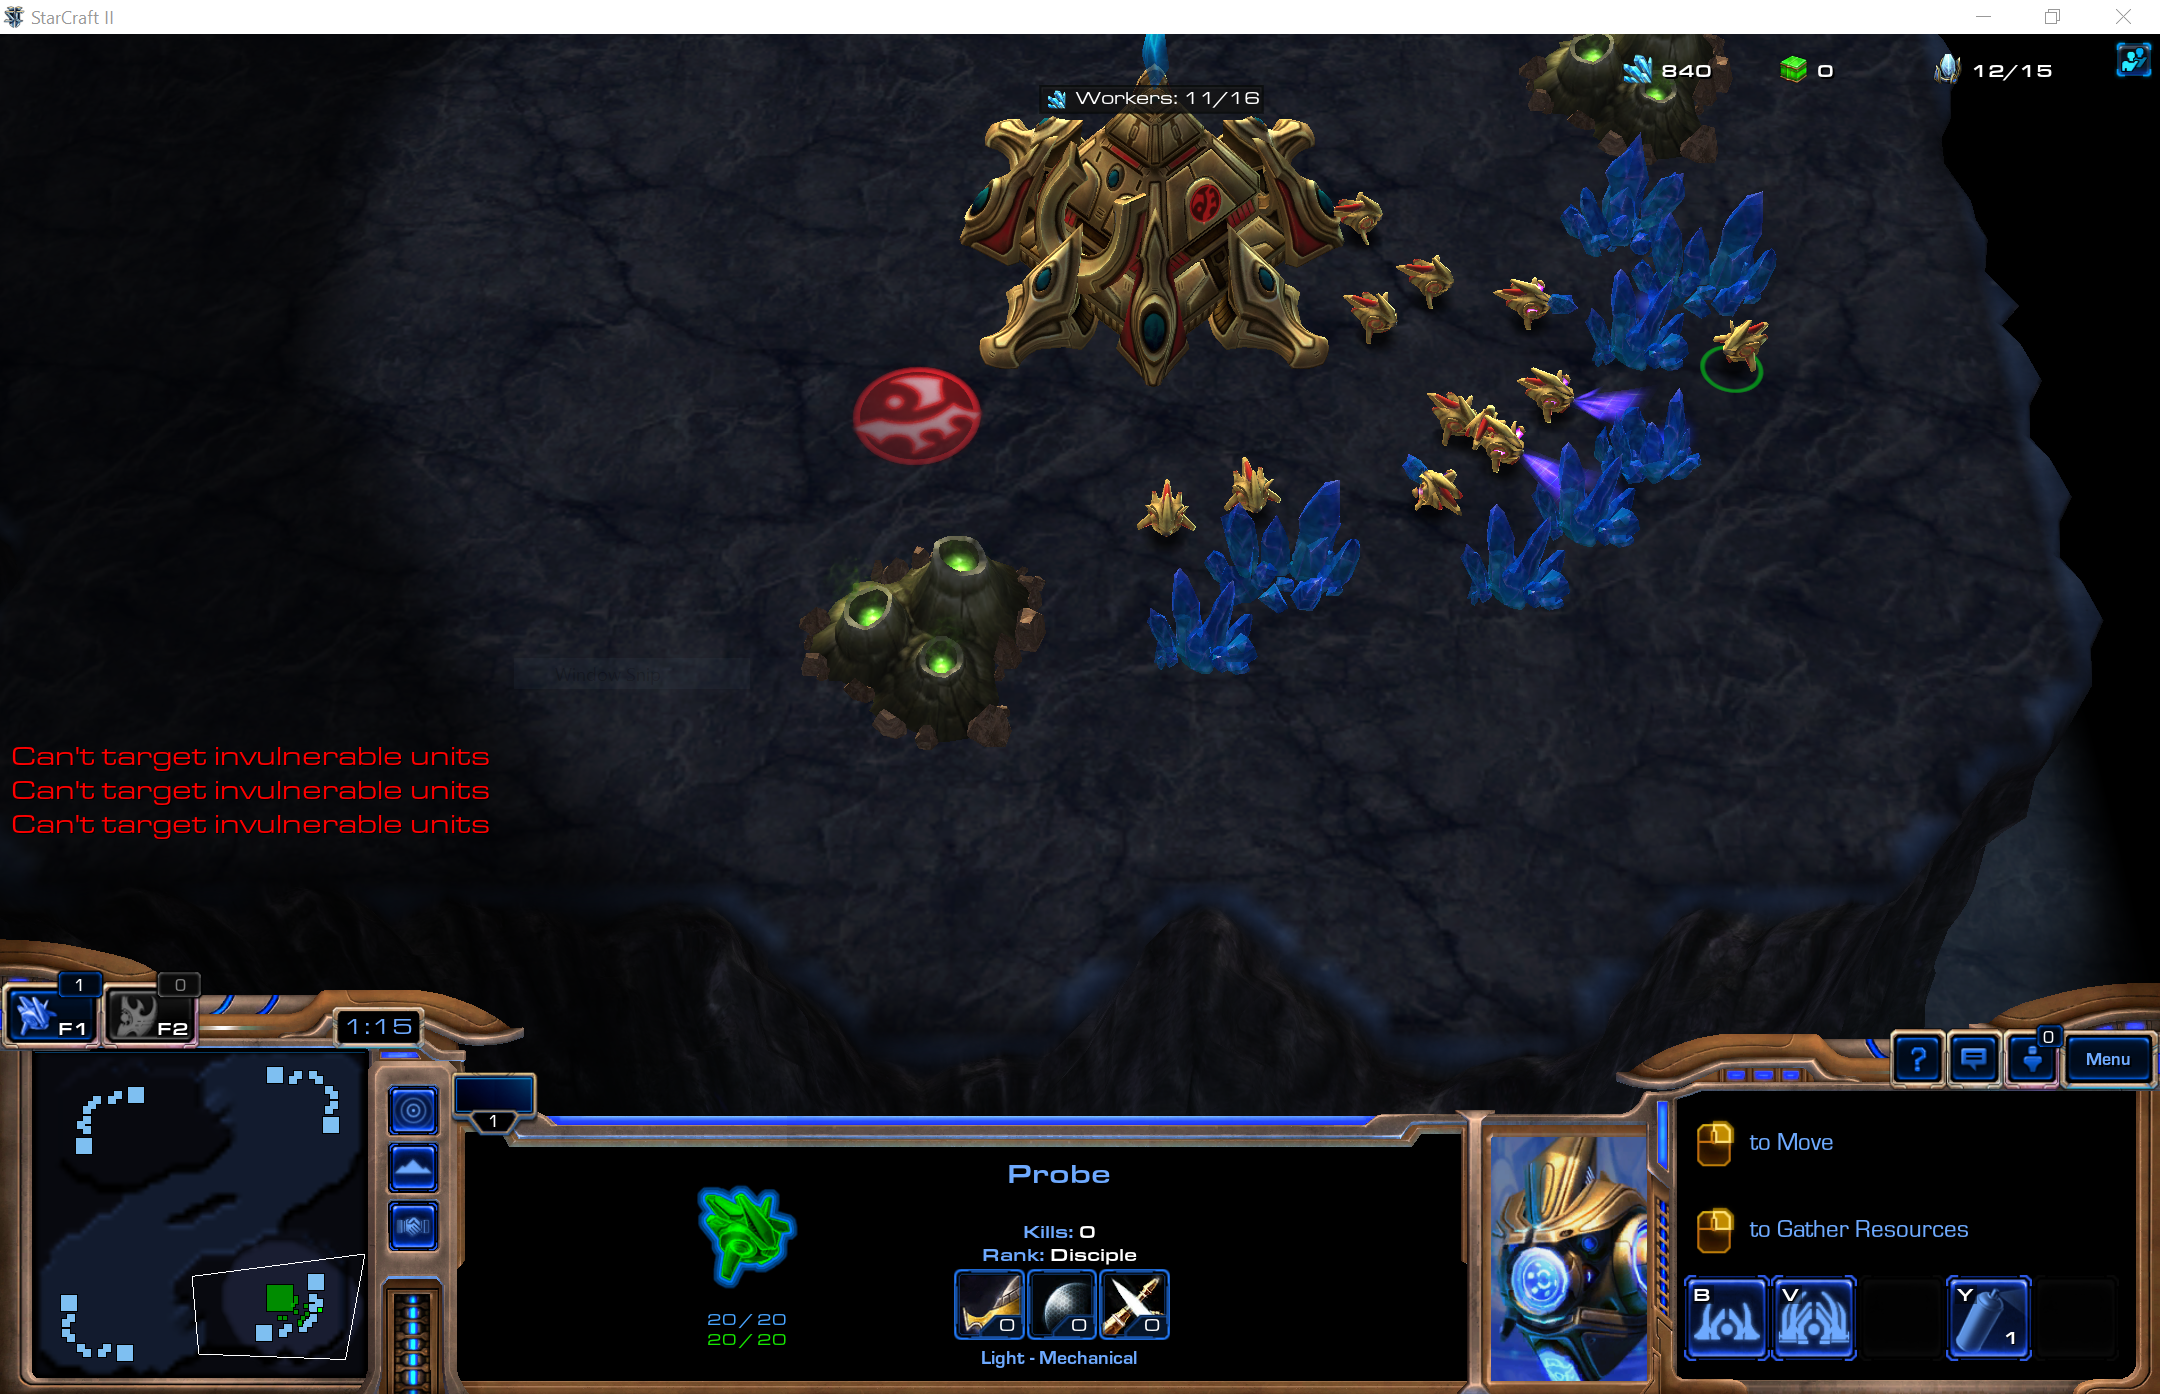
\includegraphics[width=1.0\textwidth]{scII}
    \caption{Example of the StarCraft II in-game interface.}%
    \label{fig:scII}
\end{figure}

A basic game of StarCraft II requires the management of the following:

\begin{itemize}
    \item \textbf{Resource Gathering}: Two types of resources must be gathered
        around the map, which in turn can be used to purchase additional units
        and buildings.
    \item \textbf{Unit Management}: StarCraft II consists of many
        units of varying types, which must all be given actions such that an
        efficient outcome is reached. For gathering units, this means having
        them always gathering resources of the required types or working on
        building the next required building, and for combat units
        this means controlling and utilising and their abilities effectively
        such that they are performing their best in fights. This also means
        managing the efficient spending of resources on new units.
    \item \textbf{Building Management}: Buildings must also be managed, which
        means building new buildings to either increase the maximum number of
        resources and units the player can have, or allow the building of new or
        additional number of units.
\end{itemize}

All of these actions take place on a large game map, where the player only has
partial information. That is, the player can only see the map where they have
units placed, anywhere else is shrouded in a so-called `Fog of War' which hides
any resources or enemy units which may be there. Because of this, the player
must scout the map to look for resources and the enemy, while also managing the
units and resources in their central base. In practice, this means a player is
expected to move the in-game camera back and forth around a large map, to send
and manage scouting or combat units, and jumping back to manage resource
gathering and base building at the central base.

All of these add up to many challenges for an intelligent agent to
overcome, as outlined in the next section.

Additionally, there is a significant competitive scene for StarCraft
II\cite{scIIprof}, which has a lot of potential benefits for training an
intelligent agent. It means there are many `Replays' from highly
skilled players, which could be used for supervised learning techniques, as well
as standards to compare against for unsupervised learning techniques.

\subsection{Issues with StarCraft II for an Intelligent Agent}

A game of StarCraft II includes many challenges for a player regarding
complexity. The game state can be comprised of thousands of different aspects
that could represent valuable information for the player. At a given moment,
there are potentially hundreds of different moves that a player could take,
which results in a vast action space. Plus, an average match of StarCraft II can
take between 10--15 minutes. Actions taken at the start of a game to build or
not build a potential unit type until later could result in the win or loss of a
game, meaning that every action needs to be thought out.

This means an intelligent agent for SCII would need to be able to evaluate all
these parameters too, and deal with the issues that come up in this style of
game, versus that of say Chess or Go. This will be spoken about in more detail
in Section~\ref{challenges:games}.

\subsection{Q-Learning Table}

Q-Learning is a reinforcement learning algorithm that uses a tabular approach to
state action pairs. Q-Learning is an off-policy method which gives the agent the
ability to randomly select actions in a given state without affecting the
updated value of the state action pair. Q-Learning requires:

\begin{itemize}
    \item State: some form of representation of the environment the agent is in.
    \item Action: an action that may move the agent from one state to the next
        or keep it in the same state.
\end{itemize}

The agent is given a state of the world and checks the lookup table for which
action would have the highest value in that state. The agent then executes that
action and rechecks the table again for the new state. Upon executing an action,
the agent may be given a reward, a value that dictates whether the action taken
was favorable or incorrect. The table can be updated through a real-time
learning or at the end of an episode. An episode represents an entire list of
states and actions taken to reach the end, usually by having a terminal state.
The table is updated using the Q-Learning equation. The algorithm is as follows:

\begin{itemize}
    \item The agent observes its current state
    \item The agent performs an action
    \item The agent observes the new state it is in
    \item It will also observe the new reward (if any are given)
    \item The table is adjusted for the previous state using a learning factor
\end{itemize}

The equation for updating the table is~\cite{watkins1992q}:

\begin{align}
    Q(s_t,a_t) = Q(s,a_t) + \alpha (r + \gamma (\max_a Q(s_{t+1}, a) - Q(s_t,a_t)))
\end{align}

The rewards are given as follows:

\begin{itemize}
    \item Immediate rewards: The agent is given a reward after an action is
        taken and the next state is not the final state.
        \begin{align} \label{eq:q_update}
            Q(s_t,a_t) = r + \gamma (\max_a Q(s_{t+1}, a))
        \end{align}
    \item Terminal rewards: The agent is given a reward and the state is the
        final state.
        \begin{align}
            Q(s_t,a_t) = r
        \end{align}
\end{itemize}

\subsection{Neural Networks}

Neural networks take inspiration from the biological neurons that
are present in the brain, similar to how genetic learning
algorithms take inspiration from the physical process of evolution
and mutation\cite{goldberg2006genetic}.

Broadly, a Neural Network is a model that estimates a function $f$.
It does this by using a set of weights, and input neurons. A neuron
can be thought of some model that given some inputs, gives
an output which is some weighted sum of the inputs.

A given network can have any number of neurons, connected in a number of
different ways. Typically, neurons are arranged into layers, which are sets of
neurons which are all receiving from a given input, be that an outside source,
or a different layer of neurons. An explanation of these layers will be given
later. The communication between the neurons is done by using the eights
mentioned earlier, where $w_{ij}$ denotes the weight between neurons $i$ and
$j$. Depending on the style of the network, there may be restrictions on the
values of these weights, and it is also possible that $w_{ij} \ne w_{ji}$.

For a value to be passed through the network, it is given as input to an input
layer, where it is then multiplied by the associated weights of the neuron the
value entered on, perhaps with the use of an associated activation function. A
common activation function is the Rectified Linear Unit
(RELU)\cite{Nair:2010:RLU:3104322.3104425}, which works by taking the maximum of
two values as follows:

\begin{align}
    f(x) = \max(0, x)
\end{align}

where $x$ is the input value to the activation function.

For an average network, the layout of the layers is an input layer,
followed by some hidden layers, and finally an output layer. Usually,
these layers are fully-connected, which means there every neuron in each
layer is connected to every neuron in the following layer, but
there are no connections between neurons of the layer. An example of this
is shown in Figure~\ref{fig:common_layout}.

\begin{figure}
    \centering
    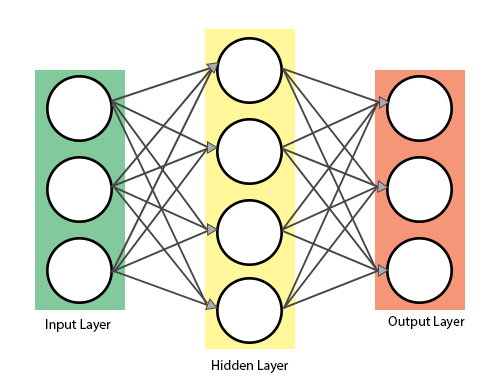
\includegraphics[width=0.6\textwidth]{common_layout}
    \caption{Common layout of a neural network.}%
    \label{fig:common_layout}
\end{figure}

\subsection{How a neural network `learns'}

For a neural network to function, it must go through a learning process, such
that it can sufficiently model the function it is needed for. This process is by
a set of functions $F$, where a solution $f' \in F$, and $f'$ solves the given
function best of all available solutions.

This leads to a need for a cost function, such that the best solution can be
found.  A cost function is defined as a mapping from the set of functions $F$ to
the real numbers, such as:

\begin{align}
    C : F \rightarrow \mathbb{R}
\end{align}

where there exists some optional solution $f^*$, which is bound as follows

\begin{align}
    C(f^*) \le C(f) \forall f \in F
\end{align}

which means that the cost of the optimal solution is bound by the cost of
all solutions in $F$.

With this, the process of the neural network learning turns into an optimisation
problem, that is, to choose the correct weights that sufficiently minimises the
cost function $C$.

The weights are picked randomly at first, before going through a tuning process
as the network is run. The specifics of this will depend on the style of network
and if a supervised or unsupervised learning method is being used, which will be
discussed later. Broadly, given these initial random weights, a training process
is used to tune the weights into being suitable. An input is received and
propagates through the network to the final output layer. Once an output is
given, it may be compared against some ground truth or metric, to evaluate if
the given output was suitable. If the output is suitable, then the next input
is received. However, if this is not the case then instead, the weights must be
adjusted, such that given the same inputs again, a more desirable result is
achieved.

Commonly, this is achieved via Backpropagation. Backpropagation is the process
of calculating the required gradient, needed to adjust the weights of the
network~\cite{goodfellow2016deep}. However, this is mainly used in supervised
learning techniques, where a known value is available.

Backpropagation is achieved through repeated use of the chain rule, to go from
the output layer back to the start of the network, using the derived gradient to
update the weights in each layer, such that they are closer to a more optimal
solution.

%TODO: Expand on backprop with more refs and explanation.

\subsection{Supervised and Unsupervised learning}

As mentioned previously, there is broadly two different styles of learning,
supervised and unsupervised learning (though there is some area between,
sometimes called semi-supervised~\cite{chapelle2009semi}).

The main differences between these two are how training is conducted. In a
supervised learning environment, there exists some dataset which has an
associated set of labels, such that learning can be done and any result can
instantly be checked against this ground truth, to help the process of
backpropagation. Unsupervised learning differs to this, where a known truth does
not exist, making the process of backpropagation much harder.

Commonly, instead the result of the outcome is instead used to help the
backpropagation process, but this can also be difficult. For example, in games
the result of an action may not be seen for hundreds or thousands of time-steps,
making the process much harder~\cite{sutton1984temporal}. This makes the
learning process harder since there is no ground truth that can be compared
against, instead, a metric that will change and adapt over a large period.

This can be avoided by using final results of a process, for example using the
result of a game, rather than the score after some number of time-steps.
However, this has other issues, such as slowing the learning process and
potentially rewarding unproductive behaviour that occurred as part of a game
that eventually was won. The opposite is also true that actions that give a
local reward may still lead to failure to win the game. Because of this, it
makes the learning process more nuanced than merely comparing against a ground
truth. This can be experimented with to see how it affects learning.

\subsection{Deep Q Networks}

The main issue with using a tabular approach to keep track of state-action
values is the number of required entries. As a more complex space needs to be
represented, the number of entries in the table would increase for every
possible combination of values. The newest approach to tackling the issue of
complex space environments is to use a neural network. The weights represent
what an expected value for a given state could be. The state is given as input
into the network, and then the highest value output is chosen as an action to be
taken by the agent. Steps for running the network are as follows:

\begin{enumerate}
    \item A state is given as input into the network.
    \item The input is multiplied by the respective connected weights.
    \item The next layer is then given the input from the previous layer.
    \item The final output layer will return different values for each node in
        the layer.
    \item The node with the highest value represents the action to be taken.
    \item Once the action is taken, a reward value is recorded and used to
        update the network.
\end{enumerate}

The main difference between a Deep Q Network and a standard neural network is
the update function used. A Deep Q Network uses the loss function from the
Q-Learning algorithm to update the weights of the network. The loss function
provides a value of the target return and the predicted return. For example, the
agent could choose that in a particular state the best action would be the third
action with a value of 20. The agent takes the action and gets a returned reward
that is less. The network is then updated to return a lesser value for that
action next time the agent is in that state again. This is known as the TD
error:

\begin{align}
    TD Error = \sqrt{{(Q(s',a) - Q(s,a))}^{2}}
\end{align}

The error is the value difference between the next state reward and the
currently expected reward. This tells the network whether the expected reward
was correct or far. The value is then updated by increasing or decreasing based
on the returned reward~\cite{pandey2010reinforcement}.

The update could be applied in real-time or at the end of every episode.

When using a real-time learning environment, the agent is more likely to mistake
an action for being optimal from the first reward it gets. This makes the agent
tend to be more bias towards actions that get an immediate return and will not
allow the agent to see the possibilities of foreshadowing what could be a better
action in the long run. To avoid overfitting for a single environment, the agent
needs to be exposed to different maps and states. Updating the network at the
end of each episode may make the agent learn action pairs that are incorrect and
do not impact the reward factor. For example, the agent can move left, which we
may assume is correct, then go right and then left again. This introduces a loop
that the agent can get stuck in or an extra action step that is unnecessary.

To avoid such an outcome, a discount factor $\gamma$ is used to reduce the
reward value for an incoming state. So the more steps an agent may take to the
reward, the lesser the reward value is. Once the agent takes an action, based on
the state given to the network, the reward is observed and used to update the
Q-Target. The Q-Target looks at the next state s' and checks which action yields
the highest value return. That value is then used to update the current state in
the network by using the TD Error.

\begin{align}
    QTarget = r + \gamma*Q(s',a)
\end{align}

The prediction made by the network is then subtracted according to the TD Error
equation. This is then multiplied by the learning rate. Final update value
is:

\begin{align}
    Q(s,a) = Q(s,a) + \alpha (TDError)
\end{align}

The equation above is the same equation used in the Q-Learning algorithm.
However, it is implemented through the network with a gradient descent
optimiser. The network evaluates the loss function using the TD Error and then
updates the relevant weights. The learning rate $\alpha$ must be tested with
multiple values. If $\alpha$ is increased then the network may converge to an
optimal value quicker but may also tend to overshoot the local minimum and
diverge from the optimal value. This makes $\alpha$ a critical hyper-parameter
based on the amount of training the agent may have. If the $\alpha$ value is set
to a lower value, then the agent will require more training to achieve an
accurate estimate of the expected reward for a given state action pair.

\subsection{Convolutional Neural Networks}

A Convolutional Neural Network (CNN) is a type of Artificial Neural Network
(ANN). Broadly, a CNN is similar to that of an ANN, in that it consists of some
neurons that have associated weights and receive some input, be that from an
input layer or another layer of neurons. Where they differ though is that with a
CNN it is assumed that the input is an image, which changes the learning
procedure and design principles.

To give an example of why this style of network is needed, the size of a non-CNN
network must be considered. For the MNIST~\cite{lecun2010mnist} dataset, the
supplied images are $28 \times 28$. For a fully connected architecture, this
leads to $28 * 28 = 784$ weights. If an RGB image is used, this number is
multiplied by 3 to get the number of pixels in each of the three channels. $784
* 3$ weights is reasonable, but once moving to an image of a more reasonable
size, say $(250, 250, 3)$, the number of weights becomes very large, without
even considering the rest of the neurons in the network.

A CNN works differently however. Since it can assume the input is an image, the
network architecture may be built in a more specific way. That is, instead of
input consisting on a flat vector of numbers, the input may be considered in 3D,
where the images vertical and horizontal resolution make up the width and height
of the input and the depth is made up of the channels the image is made up of,
traditionally 3. This is then helped further as the neurons in this 3D layer are
only connected to a small receptive field from the input image, rather than the
entire input like in a fully-connected network. Broadly, it can be said that a
convolutional layer takes a 3D input and transforms it to some 3D output. In the
context of the MNIST dataset, this would be the classification. An example of
this 3D network can be seen in Figure~\ref{fig:cnn}. It can be seen that the
image is given and is transformed into a second 3D volume of the same size, but
with additional channels.

The additional channels once the convolutional layer has been processed is due
to the number of filters in that layer. These are defined as the area the neuron
in a given layer connects to on the input. For example, a neuron in the first
layer may look at a $3 \times 3$ section of the input, extending across all
channels of the input. This filter is applied to the entire image by moving it
over every pixel combination it fits on, and at each location, the dot product
on the input and the values in the filter is computed. For the whole image $I$
and a filter $F$, this is defined as follows:

\begin{align}
    {(I*F)}_{xy} = \sum^{h}_{i=1} \sum^{w}_{j=1} F_{ij} \cdot I_{x+i-1, y+j-1}
\end{align}

which means that for a given a $(x,y)$ position, the value of the filter at that
point for a given filter is the dot product of each value in the input and the
value in the filter.

These filters are stacked, which then increases the receptive field of the later
layers. This process was mirrored on features found in
biology~\cite{hubel1968receptive}. The receptive field refers to the area that a
given neuron is receiving input from. For the first layer, this is merely the
size of the filter, for example the $3 \times 3$ grid. However, this layer is
then used as input for the next layer. It can be said that the second layer's
receptive field relative to the image for a filter of size $3 \times 3$ is
5. This increases throughout the network, building up evermore complex and
abstracted representations of the image, that are increasingly global across the
image. This can be seen in the filters that are calculated in the network,
where the earlier layers contain low-level features, where the later
ones become more abstract and cover more significant parts of the image,
as shown in Figure~\ref{fig:filter_example}.

In general, the formula a given layer $l_k$, the receptive field can be
calculated as follows:

\begin{align}
    l_k = l_{k-1} + ((f_k - 1) * \prod_{i=1}^{k-1}s_i)
\end{align}

where $f_k$ is the filter size of layer $k$ and $s_i$ is the stride for the
$i^{th}$ layer.

%TODO: Read over and check, but should be done now.

\begin{figure}
    \centering
    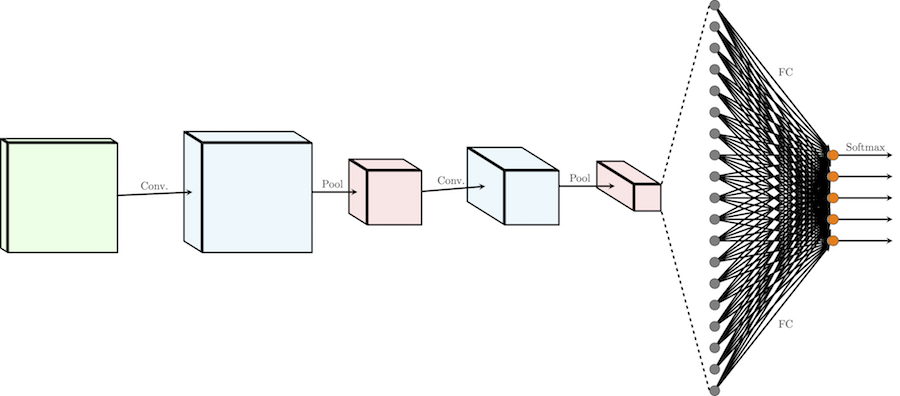
\includegraphics[width=0.9\textwidth]{cnn}
    \caption{Common layout of a convolutional neural network, from
    Cambridge Spark\cite{cnn-layout}.}%
    \label{fig:cnn}
\end{figure}

\begin{figure}
    \centering
    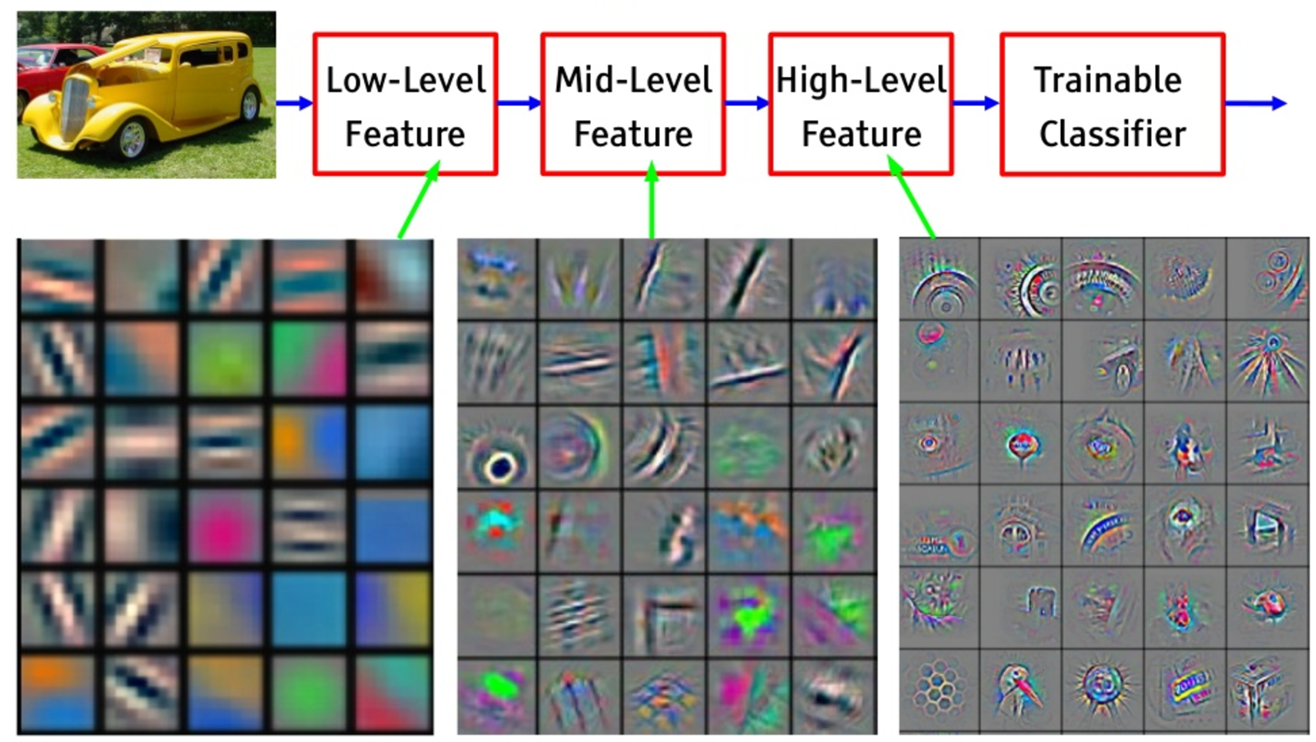
\includegraphics[width=0.9\textwidth]{filter_example}
    \caption{Examples of filters from various layers, from
    NIPS'2015 Tutorial\cite{filterexample}.}%
    \label{fig:filter_example}
\end{figure}

\subsubsection{Other required techniques}

There are other techniques that go alongside a CNN by default and have been
mentioned previously. This includes both pooling layers and the concept of
striding which is used both in the pooling layer and also the convolutional
layer.

When a filter uses a stride, the filter is moved by more than a single pixel
each time. By default, a stride is 1, that is it is applied to every single pixel
on the input. However, it is also common to have a stride of two, or in some
rare cases, a stride of greater than 2. When this is the case, the filter
is moved two pixels at a time, rather than 1. This leads to less overlap in the
receptive fields but does have the potential downside of reducing the
resolution of the input.

A pooling layer is a form of down-sampling. Given an input, the pooling layer
will reduce the resolution of it in some fashion. The most common pooling layer
used is the max-pooling layer. This layer takes the maximum value in a filter
and uses that as the value for that filter. This is commonly done with a filter
of size $2 \times 2$ and a stride of 2. The result is an image that is halved
in both the width and height dimension. This is useful to help reduce the number
of parameters in a given network, so is commonly applied after each
convolutional layer. An example of a max-pooling layer can be seen in
Figure~\ref{fig:max_pool}.

\begin{figure}
    \centering
    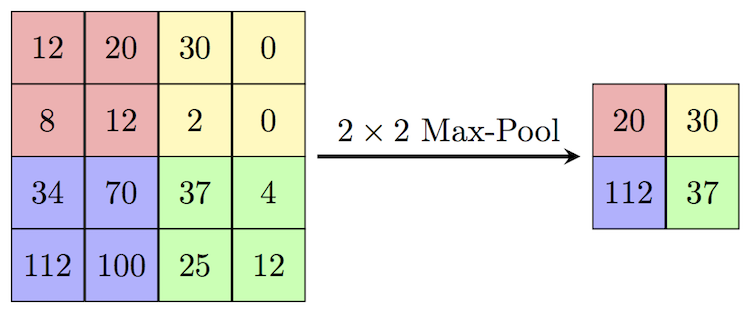
\includegraphics[width=0.9\textwidth]{max_pool}
    \caption{Example of max-pooling, from Computer Science Wiki\cite{max_pool}.}%
    \label{fig:max_pool}
\end{figure}

\subsection{Transfer Learning}

Transfer learning is a process in machine learning that describes the practice
of use knowledge learnt from one problem to help solve a different problem. The
second problem needs to be a different but related problem for transfer learning
to be useful. A typical example that is used to describe this process is that a
network that has been trained to find cars in an image could be used as the
basis of a network to locate pictures of trucks, vans or other vehicles.

Transfer learning can be useful for many reasons, the most obvious of which is
lowering the complexity of the new task, due to the network having existing
knowledge. This works best when the task at hand has not significantly changed,
but the domain has. A good example of this is the use of transfer learning in
medical applications, where knowledge in one domain can be very quickly applied
to another\cite{van2015transfer}. However, what is perhaps less obvious but more
useful, is the ability to augment an existing small dataset by using a network
trained on another domain entirely, for example using networks trained on the
ImageNet dataset\cite{ILSVRC15}, for use in entirely different domains such as
medical imaging\cite{shin2016deep, tajbakhsh2016convolutional}. This is possible
due to the task at hand, recognising some feature or object, has stayed the same
despite the vast differences in the domain.

A more formal definition of Transfer learning follows, as taken from ``A
Survey on Transfer Learning''\cite{pan2010survey}.

Given a domain $\mathcal{D}$ this is made of a feature space $\mathcal{X}$, and a
probability distribution of $P(X)$ over $\mathcal{X}$, where $X = x_1, \ldots,
x_n \in \mathcal{X}$.

A task $\mathcal{T}$ for a domain $\mathcal{D} = {\mathcal{X}, P(X)}$ consists
of $\mathcal{Y}$, a label space for the task at hand, as well as $P(Y|X)$ which
is the probability of a label $Y$ from some training data $X$, typically for
some pair $x_i \in X$ an $y_i \in \mathcal{Y}$. These labels are specific to the
domain in question, so for the MNIST dataset, they would be the numbers zero
through nine.

Finally, transfer learning can be defined as given a source domain
$\mathcal{D}_s$ with an associated task $\mathcal{T}_s$, alongside a target
domain and task $\mathcal{D}_t$ and $\mathcal{T}_t$, transfer learning aims to
learn the task of the target domain, using information from the source domain.
This is expressed as wanting to learn $P(Y_t | X_t)$ in $\mathcal{D}_t$ using
information from both $\mathcal{D}_s$ and $\mathcal{T}_s$, where either
$\mathcal{D}_s \ne \mathcal{D}_t$ or $\mathcal{T}_s \ne \mathcal{T}_t$.

This definition of the problem leads to four scenarios of transfer learning,
where each of the four elements that make up the $\mathcal{D}$ and $\mathcal{T}$
tuples are different.

%TODO: Are these 4 scenarios worth explaining?

\subsection{Curriculum Learning}

Curriculum learning is a similar process to that of transfer learning. However,
where it differs is that in transfer learning, knowledge learnt in any domain or
task is used to make a similar task easier. In curriculum learning, it is
instead the idea that learning information in a specific order can improve the
speed of convergence to some local minima, and in some cases improve the local
minima found.

This idea takes its inspiration from the fact that humans learn this way. Humans
are rarely given information in a random order; instead, they are given it in a
specific order of increasing difficulty to progress through. This can be applied
to machine learning by curating the order examples are passed to a network. This
can be as simple as preparing for training with a single small set of easy
examples, or as complicated as a full sequence of increasingly tricky cases.

Formally, this process can be defined as followed, as using the equations
outlined in ``Curriculum Learning''\cite{bengio2009curriculum}.

Given $z$, a random example for the network (or $(x, y)$ for a supervised
example and its associated label), let $P(z)$ be the target probability
distribution that would learn the required function. Let $0 \le W_{\lambda}(z)
\le 1$ be the weight applied to $z$ at step $\lambda$ in the curriculum, with
$1 \le \lambda \le 1$ and $W_1(z) = 1$. That leads to the following training
distribution at a step $\lambda$:

\begin{align}
    Q_{\lambda}(z) \propto W_{\lambda}(z) P(z) \qquad \forall z
\end{align}

such that $\int Q_{\lambda}(z) dz = 1$. This leads to

\begin{align}
    Q_1 (z) = P(z) \qquad \forall z
\end{align}

This allows us to consider an increasing sequence for $\lambda$ such that it
increases from 0 and ends at $\lambda = 1$.

This allows curriculum learning to defined as a sequence of distributions of
$Q_{\lambda}$, which we may call a curriculum if the entropy of the
distributions increases:

\begin{align}
    H(Q_{\lambda}) < H(Q_{\lambda + \epsilon}) \qquad \forall \epsilon > 0
\end{align}

and $W_{\lambda}(z)$ (the weights) are monotonically increasing (that is, always
increasing) in $\lambda$:

\begin{align}
    W_{\lambda + \epsilon}(z) \ge W_{\lambda}(z) \qquad
    \forall z, \forall \epsilon > 0
\end{align}

Broadly, this means that as we increase $\lambda$, that is by adding new
examples, $Q_{\lambda}$ also increases alongside $\lambda$, as the training
examples move from a set of small, easy examples and finishes with the full
training set. As $Q_{\lambda}$ is increasing and is proportional to the weights
and the probability distribution, the network is converging towards a better
minima.

The exact definition of what consists of an `easy example' will depend on the
domain, and can be experimented with as part of the final model's evaluation.

\section{Challenges}

Reinforcement learning has many challenges, both specific to this
project, and those that are issues for reinforcement learning as a whole.
This section aims to outline these challenges, as well as ways they have been
mitigated in other projects and how these fixes may apply to this project.

\subsection{Reinforcement Learning For Games}\label{challenges:games}

Reinforcement learning for games is particularly tricky, which is what makes it
an exciting research area. Games provide a suitable test-bed for some broader
issues in the area, while also providing a repeatable environment for running
tests.

There has been recent success playing older games using reinforcement learning,
such as games on the Atari 2600\cite{mnih2013playing} and
Doom\cite{kempka2016vizdoom}.

Both of these examples had to overcome the following issues:

\begin{itemize}
    \item `Labels': For traditional deep learning applications, a large dataset
        with associated labels is needed. However, in this case, we instead must
        learn from a reward, which is usually delayed for a number steps. For
        example, a reward may not be given until the game is finished, in which
        case it is tough to link early actions to the reward. The first
        action taken could have a strong correlation or no effect on the final
        score, but tracking it over an entire game can prove very difficult.
    \item Independence of Inputs: Most deep learning algorithms assume that
        all inputs are independent, which is usually not the case for
        reinforcement learning. This is usually because in reinforcement
        learning each state follows the last, in this case as frames of input
        from the game. This can cause issues due to the network needing to
        understand that a given state leads to another and so on.
    \item Action Space: In games, there is usually a vast number of actions that
        a player can take at any given moment. This can be in the form of either
        the number of actions or the number of locations a given action can
        take place at. Shooting at one spot is not the same as shooting at
        another. This usually means that both an action and location pair is
        required.
    \item Incomplete Information: Unlike in most forms of supervised learning,
        reinforcement learning commonly has elements of incomplete information,
        that is there is missing information. This is not always the case, such
        as in Go or Chess, but most games have elements of missing information.
        This makes it more difficult to decide since the full state is
        not available.
\end{itemize}

However, there are also things which are much easier to use in reinforcement
learning, such as learning with self-play that is having an agent play against
another agent. This has been used in Poker\cite{heinrich2016deep}, Chess and
Shogi\cite{silver2017mastering} and most recently
Go\cite{silver2016mastering,silver2017masteringgo} to great success.


\subsection{StarCraft II specific issues}

StarCraft II specifically offers an environment that offers a lot of interesting
challenges.

First, there is the issue of associating a reward with an action. This is
especially an issue for StarCraft II for a few reasons. The main of which is
the rate at which actions are taken is incredibly high, especially in high-level
play. Professional players can hit upwards of 150 actions-per-minute
(APM)\footnote{Value is taken from:
\url{http://starcraft.wikia.com/wiki/Actions_per_minute}}, which over an average
game of 10--15 minutes, combines to numerous actions that need to be given and
later have a given reward associated with them. This can be avoided if a supervised
learning approach is taken. As mentioned previously, there are many `game
replays' available, from all styles of games. These replays contain the full
game and all actions taken, so can be used to either augment a reinforcement
learning approach, either through starting a network or helping an existing
network learn. This approach has been used to varying success in similar domains
such as Atari games\cite{hester2018deep} and also the original StarCraft
game\cite{justesen2017learning}.

Replays also help the second issue, which is incomplete information.
A game of StarCraft II takes place on a potentially large map, with up to 8
players simultaneously playing on the standard maps. This means that an agent
could be missing out on the information of 7 other players. Both the number of
players and the size of the maps lead to a significant amount of missing information.
However, replays do not have this restriction, and as such both players and bots
alike can use replays to analyse both their own and other players strategies to
improve their play.

Similarly, due to the large map and the wide range of units in the game, there
is a significantly large action space at any given time. Compared to a game like
Chess, where there is a (comparatively) small number of units, actions and
spaces to perform those actions, SCII has an order of magnitude more actions
available, meaning an agent has more options they must perform. Similarly, there
are many moves that require complex planning, such as `Build a
combat unit', which may take many steps to reach, such as gather
resources to some amount, build a building to build that specific unit, wait for
the building to be complete, and finally, queue the building of the required
unit. This sequence of actions and more complicated ones need to be learnt to
be a successful SCII player.

Additionally, compared to a game such as chess or even the Atari games,
StarCraft II consists of multiple in-game characters which must be controlled.
In Chess, a single piece is moved each turn normally, whereas in StarCraft II a
group of units must be moved, which means selecting the required units and
moving them. This complicates the movement action as it is now depends on a
selection step. This is made more complicated due to the limitations of the API
making selecting certain units from a group much harder.

\section{Existing Methods}

There are many existing methods in the area of reinforcement learning for games,
as well as solutions that fall outside of gaming but are still potentially
relevant.

For example, there is existing research into applications for the original
StarCraft game, where some different methods were tested. The methods vary
wildly, and a few examples are given now.

The paper ``Reinforcement learning agents providing advice in complex video
games''~\cite{taylor2014reinforcement} talks about using a system to train a
network, given guidance from a teacher. It discusses the use of having a network
be a `student' such that it takes instructions from the teacher as it learns to
guide its learning, though this process can only be used a certain number of
times. The conclusion reached shows that given suitable advice, an agent can
learn much faster. While interesting, this style of learning is not readily
compatible with the use of curriculum or transfer learning, which limits its
usefulness in this project. However, it could be an exciting extension in the
future.

There are many papers on the use of reinforcement learning for the original
StarCraft game and its expansions~\cite{wender2012applying,
shantia2011connectionist}. However, many of these solutions had issues with the
processing of the system, such that they had to develop novel systems to even
get the data out efficiently, which is not a problem with the SC2LE\@. Despite
these issues, they managed to get intelligent behaviour out of the respective
agents either in full games or in small problems that were subsets of the full
game. Both of these agents used a Q-Learning approach or a Sarsa learning
approach~\cite{sutton1996generalization} to differing results. The results
achieved as well as the methods used could prove useful informing design
decisions for the networks used for this problem. However, due to the change in
both the game and the method that is used to interact with the game, the
techniques and parameters used could prove to be less useful due to a
significant difference in the two environments.

Finally, the last area that can be used for inspiration is the vast amount of
work that has been done in the field of reinforcement learning throughout gaming,
rather than the work that is specific to StarCraft. While older games such as
the Atari 2600 games mentioned above, differ massively from StarCraft, there are
more modern games that have similar problems. For example, the game
Civilization IV~\cite{wender2008using}, which is a complicated strategy game,
taking place over a map that covers a large number of playable spaces, with
games taking many thousands or millions of steps potentially, depending on the
game settings. As such, similarly to StarCraft, the game has significant issues
with associating rewards and choosing the location that actions should be taken
at. As a result, most research is done on small subsets of the game. This
strategy again uses Q-Learning and could provide useful insights into the
design for a network for StarCraft II\@.

%TODO: Potentially needs more stuff on other games in the last paragraph.

\section{Formal Definition of the Problem}

The final part of the research was into the problem of creating an intelligent
agent for StarCraft II\@. The previous sections cover all the technical aspects
that would be needed for such an agent, but does not attempt to define what
consists of an intelligent agent, nor what is required to consider the project a
success.

As mentioned, the game of StarCraft II consists of many elements, such that the
scope of an intelligent agent must be restricted, for it to remain feasible.
Because of this, the game will focus on two specific tasks: The DeepMind
mini-games and the Simple64 map. Both of these are explained in more detail in
Chapter~\ref{implem}.

Intelligent behaviour is hard to define, due to the inherent subjectivity in
determining what it consists of. This is spoken about in more detail as part of the
Evaluation Methodology in Chapter~\ref{eval_method}, but broadly the definition
used for this project is that intelligent behaviour is taking the most direct
route to a given solution or state possible, without having too many superfluous
actions. This means an agent does not necessarily need to reach a most optimum
state, as it is also true that many humans play games sub-optimally. However,
the agent should still efficiently move to that state.

To give a more structured example, consider a single agent has to move to
a set location. It may be quickest to follow a specific path, but the agent's
behaviour will be regarded as intelligent if it can move directly to the
target location, without unneeded actions such as turning around or attacking at
random on that path. The agent does not necessarily need to follow the optimal
path, but for such a simple example it could be expected that it would. This
expectation, however, would change depending on the complexity of the task.

\subsection{Solution Choices}

From the research that went into this chapter and the associated similar
problems, two styles of a solution will be built and tested.

First, a Q-Learning approach will be taken. This approach has been tested across
many different games and should prove very useful for this task. If combined
with compound actions that combine multiple actions into one single agent
action, it is possible that an agent may be able to show intelligent behaviour
across the many different test situations, to give a strong result. This
approach has the advantage of being used very readily across a vast number of
projects, including StarCraft and StarCraft II projects, as well as many other
games.

Secondly, a Convolutional Neural Network approach will be taken. This approach
has less testing, but a form of CNN did behave the best in the DeepMind SC2LE
paper~\cite{vinyals2017starcraft}, so there is proven results in the area that
show a CNN performs very well at this task. This approach should be more global
since it takes input of the entire visual space, and perhaps other additional
information, to learn its environment sufficiently.  However, it is also
possible that due to the higher complexity of being forced to select more
specific actions instead of the Q-learning approaches compound actions, it may
fair worse for tasks that require large amounts of tasks that take multiple
steps.

Both of these networks will allow research into Transfer and Curriculum
learning, such that their effect on both the learning speed as well as the agent
efficiency can be measured and compared.

Using the insights the many past projects gained should mean that a solution
can be found that avoids the issues outlined in~\ref{sc2-issues}. This mix of
solutions should also give an interesting comparison between the different
learning styles, and how each one fair for a given challenge.

\section{Conclusion}

In conclusion, this chapter has formally defined the required theory behind
neural networks, as well as both Deep Q networks and Convolutional Neural
Networks. Following this was an evaluation of the challenges the project could
face as well as the methods that have been attempted in and around the area,
such that they also may be considered here. Finally, a formal definition of the
problem and the solution choices based on the research gathered was given.

The network styles were chosen due to their proven results in the area, across
multiple games and project styles. These existing projects and deeper
understanding of the project area should give the created solutions more depth
and allow more informed decisions to be taken, as well as avoiding pitfalls that
may have been met otherwise.

Following this research, preliminary designs for networks can be made, to allow
the testing of the methods outlined here, as well as the later evaluation of
their performance, with a better idea of what constitutes an intelligent agent.
The following chapter will go into details of the design choices that went into
the design of the final networks, before outlining the performance metrics and
the achieved results.
